\section{Aritmetica}
\subsection{Priorità delle operazioni}
\begin{questions}


\question
\exonly{	Calcola senza aiutarti con la calcolatrice:}

\begin{minipage}{\linewidth}
	\begin{multicols}{3}
		\begin{parts}
			\part 
			\exonly{$ \frac{2}{3} + \frac{3}{4} = $ } 
			\solonly{ $\frac{17}{12}$  }
			\part 
			\exonly{$ \frac{7}{6} - \frac{5}{8} + \frac{4}{9} = $ }
			\solonly{$\frac{71}{72}$ }
			\part 
			\exonly{$ \frac{1}{15} - \frac{2}{5} + \frac{3}{25} = $ }
			\solonly{$-\frac{16}{75}$ }
			\part 
			\exonly{$ \frac{2}{6} + \frac{5}{15} - \frac{12}{18} = $ }
			\solonly{$0$ }
			\part 
			\exonly{$ \frac{a}{3} + \frac{2}{5} - \frac{4}{3} = $ }
			\solonly{$\frac{5a-14}{15}$ }
			\part 
			\exonly{$ \frac{1}{x} + \frac{3}{5} - \frac{3}{2x} = $ }
			\solonly{$\frac{6x-5}{10x}$ }
			\part 
			\exonly{$ \frac{\frac{1}{3} + \frac{1}{5}}{\frac{4}{15}-\frac{2}{6}} = $}
			\solonly{$-8 $ }
			
			\part 
			\exonly{$ \frac{\frac{2}{3} \cdot (\frac{1}{6} +  \frac{1}{2})}{\frac{3}{4}-\frac{3}{10}} = $}
			\solonly{$\frac{80}{81}$ }
			
			\part 
			\exonly{$ \frac{2}{3} \cdot \frac{1}{5} + \frac{\frac{3}{2}}{\frac{7}{5}} = $ }
			\solonly{$\frac{253}{210}$ }
			
			\part 
			\exonly{$ \frac{4}{9} \cdot \frac{6}{10} + \frac{\frac{8}{30}}{\frac{6}{5}} = $ }
			\solonly{$ \frac{22}{45}$ }
		\end{parts}	
\end{multicols} 
\end{minipage}


\exonly{\vspace*{\stretch{1}} }


\question
\exonly{Calcola senza aiutarti con la calcolatrice:}
	
	\begin{minipage}{\linewidth}
	\begin{multicols}{2}
		\begin{parts}
			\part 
			\exonly{$ 2^3 \cdot 2^{-2} \cdot 2^4 \cdot 2^{-1} =$ }
			\solonly{$16 $ }
			
			\part 
			\exonly{$ \dfrac{3^2\cdot 3^3}{3^4} = $ }
			\solonly{$3 $ }
			
			\part 
			\exonly{$ \dfrac{5^3\cdot 5^{-2}}{5^4 \cdot 5^{-3}} = $ }
			\solonly{$1$ }
			
			\part 
			\exonly{$ \left(2^2\right)^2 \cdot \left(2^{-1}\right)^3 \cdot \left(2^2\right)^{-2} $ }
			\solonly{$\frac{1}{8} $  }
			
			\part 
			\exonly{$ \left(3^2\right)^{-1} \cdot \left(2^{-2}\right)^{-1} \cdot \left(6^2\right)^2 =$ }
			\solonly{$576 $ }
			
			\part 
			\exonly{$ \left[\left(\dfrac{1}{5}\right)^{2}\cdot\left(\dfrac{1}{5}\right)^{3}\right]^{2}\cdot\left(\dfrac{1}{5}\right)^{-7} = $ }
			\solonly{$ \frac{1}{125}$  }
			
			\part 
			\exonly{$ \dfrac{3^5 \cdot 2^4}{6^3} = $ }
			\solonly{ $18$  }
			
			\part 
			\exonly{$ \dfrac{\left[\left(\dfrac{3}{4}\right)^{-1}\right]^{2} \cdot \left(\dfrac{2}{9}\right)^{-2}}{\left(\dfrac{1}{6}\right)^{-3}} = $ }
			\solonly{$\frac{1}{6} $ }
			
			\part 
			\exonly{$ \left\lbrace \dfrac{\left[\left(3^{2}\right)^{-1}\right]^{2}}{\left(\dfrac{1}{3}\right)^{-3}}\right\rbrace ^{-1} \cdot \left[\left(\dfrac{2}{5}\right)^{2} \cdot \left(\frac{5}{6}\right)^{2}\right]   = $ }
			\solonly{$ 243$ }
		\end{parts}
	\end{multicols}
\end{minipage}


\vspace*{\stretch{1}}

\question
\exonly{Semplifica e calcola senza utilizzare la calcolatrice: }

%\exonly{
%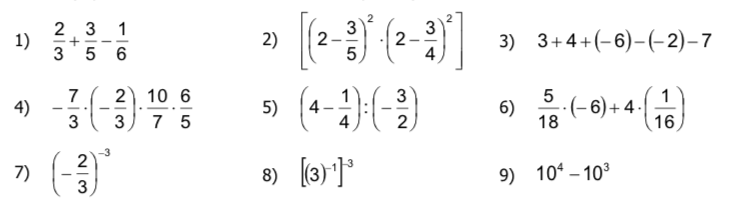
\includegraphics[scale=0.6]{test-form-1}
%
%}
\begin{minipage}{\linewidth}
	\begin{multicols}{2}
		\begin{parts}
			\part
			\exonly{$\frac{2}{3}+\frac{3}{5}-\frac{1}{6}$ }
			\solonly{$\frac{11}{10}$ }
			
			\part
			\exonly{ $\left[ \left( 2-\frac{3}{5}\right) ^2 \cdot \left( 2-\frac{3}{4}\right) ^2 \right] $  }
			\solonly{$\frac{49}{16}$ }
			
			\part
			\exonly{$3+4+(-6)-(-2)-7$ }
			\solonly{$-4$ }
			
			\part
			\exonly{$-\frac{7}{3} \cdot \left( -\frac{2}{3}\right) \cdot \frac{10}{7} \cdot \frac{6}{5} $ }
			\solonly{$\frac{8}{3}$ }
			
			\part
			\exonly{$\left( 4-\frac{1}{4}\right) \div \left( -\frac{3}{2}\right) $ }
			\solonly{$-\frac{5}{2}$ }
			
			\part
			\exonly{$\frac{15}{18}\cdot\left( -6 \right) +4\cdot \left( \frac{1}{16}\right) $ }
			\solonly{$-\frac{19}{4}$ }
			
			\part
			\exonly{$\left( -\frac{2}{3}\right) ^{-3}$ }
			\solonly{$-\frac{27}{8}$ }
			
			\part
			\exonly{$\left[ \left( 3\right) ^{-1}\right] ^{-3}$ }
			\solonly{$27$ }
			
			\part
			\exonly{$10^4-10^3$ }
			\solonly{$9000$ }
		\end{parts}
	\end{multicols}
\end{minipage}


\vspace*{\stretch{1}}

\question
\exonly{Calcola senza aiutarti con la calcolatrice:}

\begin{minipage}{\textwidth}	
		
		\begin{multicols}{2}
			\begin{parts}
				
				\part 
				\exonly{$ x - 2x + 3x - 4x + 5x - 6x =$ }
				\solonly{$ -3x$ }
				
				\part 
				\exonly{$ a^2 + 2a -3a^2 +a = $ }
				\solonly{$-2a^2+3a$ }
				
				\part
				\exonly{$ a^2 \cdot a^3 = $ }
				\solonly{$a^5$ }
				\part 
				\exonly{$ \left(a^2\right)^2 + a\cdot a^3 - \left(a^6\right)^{-2} =$ }
				\solonly{$\dfrac{2a^{16}-1}{a^{12}}$ }
				
				\part 
				\exonly{$ x^{-2} \cdot \left(x^2\right)^3 = $ }
				\solonly{$x^4$ }
				
				\part 
				\exonly{$ \dfrac{9 \cdot a^2 \cdot b^3 }{3 \cdot a^{-2} \cdot b^5} = $ }
				\solonly{$\dfrac{3a^4}{b^2}$ }
				
				\part 
				\exonly{$ \dfrac{2 \cdot a^3 \cdot b^2 }{3 \cdot a \cdot b^4} \cdot \dfrac{a+b}{a}  = $ }
				\solonly{$\dfrac{2a^2+2ab}{3b^2}$ }
				
				\part 
				\exonly{$ a\left(a(a^{-1}+1) + a(a-1)\right) =$ }
				\solonly{$ a^3+a$ }
			\end{parts}
			
		\end{multicols}
		
\end{minipage}


\end{questions}

\exnewpage

\subsection{Notazione scientifica}
\begin{questions}

\question
\exonly{Esprimi la tua altezza in notazione scientifica}
\solonly{Esempio con \SI{178}{\centi\metre} }

	\begin{multicols}{2}
		\begin{parts}
			\part 
			\exonly{in metri }
			\solonly{ \SI{1.78}{\metre} }
			\part 
			\exonly{in centimetri }
			\solonly{\SI{1.78e2}{\centi\metre} }
			\part 
			\exonly{in millimetri }
			\solonly{\SI{1.78e3}{\milli\metre} }
			\part 
			\exonly{in chilometri }
			\solonly{\SI{1.78e-3}{\kilo\metre} } 
			\part 
			\exonly{in pollici ($\SI{1}{in}=\SI{2.54}{cm}$) }
			\solonly{\SI{7.01e1}{in} }
			\part 
			\exonly{in piedi ($\SI{1}{ft}=\SI{12}{in}$) }
			\solonly{\SI{5.84}{ft} }
		\end{parts}
	\end{multicols}


\vspace*{\stretch{1}}


\question
\exonly{Calcola senza aiutarti con la calcolatrice:}

	\begin{parts}
		\part 
		\exonly{$\num{2e3} + \num{5e2} +\num{3e1}=$ }
		\solonly{\num{2530}=\num{2.53e3} }
		\part
		\exonly{ $\num{3e3} + \num{5e-2} +\num{2e-1} + \num{6e1} + \num{4e0} + \num{9e2} + 7 \times 10^0=$ }
		\solonly{\num{3971.25} }
		
		\part 
		\exonly{$ \num{12e3} \times \num{2e-3} \times \num{3e-6} =$ }
		\solonly{\num{72e-6}=\num{7.2e-5} }
		
		\part 
		\exonly{$ \dfrac{\num{12e3}+ 500}{\num{5e6}} = $ }
		\solonly{ \num{2.5e-3}  }
		
		\part 
		\exonly{$ \dfrac{\num{2e-2} \times\num{3e1} \times\num{4e2}}{\num{4e2} \times\num{6e-3} \times\num{2e1}} =$ }
		\solonly{ \num{5}}
		
	\end{parts}


\vspace*{\stretch{1}}


\question
\exonly{ Calcolare le seguenti espressioni ed esprimere il risultato in notazione scientifica }

\begin{minipage}{\linewidth}
	\begin{multicols}{2}
		\begin{parts}
			\part
			\exonly{ $\num{0.5e-1 }$ }
			\solonly{$ \num{5e-2}$ }
			
			\part
			\exonly{ $\num{-6.5e-5} -\num{3.5e-7} $ }
			\solonly{$-\num{6.535e-5} $ }
			
			\part
			\exonly{$\left(3 \cdot 10^{-2}\right)\left(4 \cdot 10^{-1}\right)$ }
			\solonly{ $\num{1.2e-2}$ }
			
			\part
			\exonly{$8^{2} \cdot 10^{-2}$ }
			\solonly{$\num{6.4e-1} $ }
			
			\part
			\exonly{ $200 \cdot 10^{4}$ }
			\solonly{$\num{2e6}$ }
			
			\part
			\exonly{$\left(5 \cdot 10^{-4}\right)\left(0,7 \cdot 10^{-8}\right)$ }
			\solonly{$\num{3.5e-12} $ }
			
			\part
			\exonly{$\left(7 \cdot 10^{-7}\right)^{2}$ }
			\solonly{$\num{4.9e-13}$ }
			
			\part
			\exonly{ $\left(3^{2} \cdot 10^{-6}\right)^{2} \cdot 10$ }
			\solonly{$ \num{8.1e-10} $ }
			
			\part
			\exonly{$10^{4}-10^{3}$ }
			\solonly{$\num{9e3}$ }
			
			\part
			\exonly{ $\left(0,4 \cdot 10^{-4}\right)(0,8) \cdot 10^{-4}$}
			\solonly{$\num{3.2e-9}$ }
			
			\part
			\exonly{$10^{5}-10^{-5}$ }
			\solonly{$\num{9.999999999e4}$ }
			
			\part
			\exonly{$\frac{\left(4^{2}\right)^{-2} \cdot 10^{-3}}{4^{-2} \cdot 10^{-8}}$ }
			\solonly{ $\num{6.25e3}$ }
			
			\part
			\exonly{$-\num{4.2e-3}+\num{4.2e5}$ }
			\solonly{$\num{4.199999958e5} $ }
		\end{parts}
	\end{multicols}
\end{minipage}


\vspace*{\stretch{1}}


\question
\exonly{Calcola ed esprimi il risalutato tenendo conto delle cifre significative delle misure:}

\begin{minipage}{\linewidth}
	\begin{multicols}{2}
		\begin{parts}
			\part 
			\exonly{$ \SI{5.3}{cm} - \SI{3.2}{mm} = $  }
			\solonly{\SI{50}{\milli\metre}=\SI{5.0}{\centi\metre} }
			\part 
			\exonly{$ \SI{43.5}{cm} \cdot \SI{9.3}{mm} = $  }
			\solonly{\SI{4.0e1}{\square\centi\metre}=\SI{4.0e3}{\square\milli\metre} }
			\part
			\exonly{ $ \SI{9.2}{cm^2} + \SI{123}{mm^2} = $  }
			\solonly{ \SI{1.0e3}{\square\milli\metre} }
			\part
			\exonly{ $ \dfrac{\SI{430}{mm^2}}{\SI{3.2}{cm}} = $ }
			\solonly{$\SI{1.3e1}{mm}$ }
			\part 
			\exonly{$ \SI{3.2}{k\ohm} \cdot \SI{15}{mA} = $ }
			\solonly{$\SI{48}{V}$ }
			\part 
			\exonly{$ \dfrac{\SI{12}{V}}{\SI{60}{mA}} = $ }
			\solonly{\SI{2.0e2}{\ohm} }
		\end{parts}
	\end{multicols}
\end{minipage}


\vspace*{\stretch{1}}


\question
\exonly{
	Esprimi le seguenti frazioni in notazione scientifica e tecnica tendendo conto delle cifre significative }

\begin{minipage}{\linewidth}
	\begin{multicols}{2}
		\begin{parts}
			\setlength\itemsep{1em}
			\part 
			\exonly{$\frac{5}{8}$ }
			\solonly{\num{6e-1} \\ \num{600e-3} }
			\part 
			\exonly{$\frac{724}{5}$ }
			\solonly{\solonly{\num{1e2} \\ \num{100e0} } }
			\part 
			\exonly{$\frac{11562}{470000}$ }
			\solonly{\num{2.5e-2} \\ \num{25e-3} } 
			
			\part 
			\exonly{$\frac{123456}{7}$ }
			\solonly{ \num{2e4} \\ \num{20e3}  }
			
			\part
			\exonly{ $\frac{12}{16500}$= }
			\solonly{\num{7.3e-4} \\ \num{730 e-6}  }
			
			\part 
			\exonly{$\frac{146}{2420}$= }
			\solonly{\num{6.03e-2} \\ \num{60.3e-3}  }
		\end{parts}
	\end{multicols}
\end{minipage}


\end{questions}
